\documentclass[11pt,a4paper,english]{article}
  \usepackage[latin1]{inputenc}
  \usepackage{amsmath,amsfonts,amssymb}
  \usepackage{enumitem}
  \usepackage{fullpage}
  \usepackage{graphicx}
  \usepackage{tabto}
  \usepackage{etoolbox}
  \usepackage{hyperref}
  \usepackage{minted}
  \usepackage{parskip}
  \usepackage[title]{appendix}
  \graphicspath{ {./} }

  \title{Bayesian Data Analysis - Assignment 2}
  \author{}

  \begin{document}
    \maketitle
    \definecolor{bg}{rgb}{0.95,0.95,0.95}

    Before responding to questions a, b, c and d; we have to calculate prior
    and posterior values. From the description and provided data we know that
    there are 274 lakes, from which 230 did not show any algae sign and 44 of
    them had algae.

    \begin{math}
      \textbf{P(algae\ exist\ based\ on\ data)} = \dfrac{44}{274} = 0.1605\\
      \textbf{prior} = Beta(2,10) = \dfrac{2}{2+10} = 0.166\overline{6}\\
      \textbf{posterior} = Beta(
        positive(prior + data), negative(prior + data)
      ) = Beta(2+44, 10+230)\\
        = \dfrac{46}{240} = 0.1608
    \end{math}

    \begin{enumerate}[label=\alph*.]
      \item \textit{Summarize:}\\
        Based on the graph that depicts the probability distribution of prior
        and posterior we can conclude that the data makes posterior more
        explicit and concrete.
        It can be easily observed that the value of $\pi$ has a higher probability
        in the intervals: \textbf{[0.096, 0.235]}.
        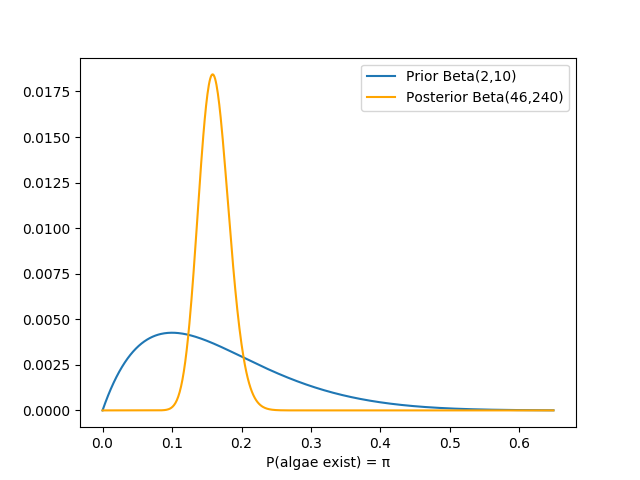
\includegraphics[width=10cm]{prob_distribution.png}

      \item \begin{math} P(\pi_0 = 0.2): \end{math}\\
        The probability that the proportion of monitoring sites with detectable
        algae levels $\pi$ is smaller than $\pi_0$ = 0.2 is equal to \textbf{0.9586}.
        which can be calculate like
        \begin{minted}[bgcolor=bg,fontsize=\small,autogobble]{python}
          stats.beta.cdf(0.2, a=46, b=240)
        \end{minted}
        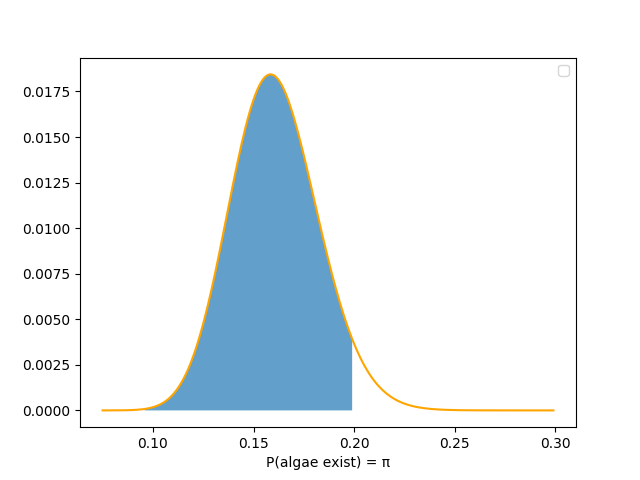
\includegraphics[width=10cm]{cumulative.png}

      \item \textit{What are the required assumptions:}\\
        All lakes have the same distribution and expected value.

      \item \textit{Make prior sensitivity analysis:}
        \\
        \begin{math}
          B(1,5) = \dfrac{1}{1+5}=0.16\overline{6} $\tab$ posterior=0.160\\
          B(20,100) = \dfrac{20}{20+100}=0.16\overline{6} $\tab$ posterior=0.162\\
          B(40,200) = \dfrac{40}{40+200}=0.16\overline{6} $\tab$ posterior=0.163\\
          B(60,300) = \dfrac{60}{60+300}=0.16\overline{6} $\tab$ posterior=0.164
        \end{math}

        The above calculation shows the sensitivity of posterior inference
        about $\pi$ to the proposed prior distribution. It uses use prior
        distributions that are increasingly concentrated around 0.162,
        the proportion of lakes with algae.
    \end{enumerate}

    \begin{appendices}
      \section{Source code}
      \begin{minted}[bgcolor=bg,linenos,fontsize=\small,autogobble]{python}
        from scipy import stats
        import numpy
        import matplotlib
        matplotlib.use('TkAgg')
        import matplotlib.pyplot as plt

        # a) summarize
        x_range = numpy.arange(0, 0.65, 0.001)
        prior = stats.beta.pdf(x_range, a=2, b=10)/1000
        posterior = stats.beta.pdf(x_range, a=46, b=240)/1000

        plt.plot(x_range, prior, label='Prior Beta(2,10)')
        plt.plot(x_range, posterior, label='Posterior Beta(46,240)', color='orange')

        plt.xlabel('P(algae exist) = pi')
        plt.legend()
        plt.savefig('./ex2/report.tex/prob_distribution.png')
        plt.show()

        # a) P(pi0= 0.2)
        cumulative = stats.beta.cdf(0.2, a=46, b=240)
        print('cumulative at 0.2: ', cumulative)

        x_range2_line = numpy.arange(0.075, 0.3, 0.001)
        posterior2_line = stats.beta.pdf(x_range2_line, a=46, b=240)/1000

        x_range2 = numpy.arange(0.096, 0.2, 0.001)
        posterior2 = stats.beta.pdf(x_range2, a=46, b=240)/1000

        plt.fill_between(x_range2, posterior2, alpha=0.7)
        plt.plot(x_range2_line, posterior2_line, color='orange')

        plt.xlabel('P(algae exist) = pi')
        plt.legend()
        plt.savefig('./ex2/report.tex/cumulative.png')
        plt.show()
      \end{minted}
    \end{appendices}
\end{document}
